\documentclass[12pt]{article}
\parindent=0.25in

\setlength{\oddsidemargin}{0pt}
\setlength{\textwidth}{440pt}
\setlength{\topmargin}{0in}
\usepackage{amssymb}
\usepackage{amsfonts}
\usepackage{amsmath}
\usepackage{cancel}
\usepackage{latexsym}
\usepackage[center]{subfigure}
\usepackage{epsfig}
\usepackage{3952}
\usepackage{3952-thm}
\usepackage{pstricks,pst-node,pst-tree}
\usepackage{soul, xcolor}
\usepackage{bbold}
\usepackage[backref, colorlinks,citecolor=blue,bookmarks=true]{hyperref}  


% \def\size{\mathop{\rm{size}}\nolimits}
% \def\depth{\mathop{\rm{depth}}\nolimits}
% \newtheorem{theorem}{Theorem}
% \newtheorem{lemma}{Lemma}
% \newtheorem{corollary}{Corollary}
% \newtheorem{fact}{Fact}
% \newtheorem{definition}{Definition}
% \newtheorem{claim}{Claim}
% \newenvironment{proof}{\noindent \textbf{Proof:}}{$\Box$}
% \newenvironment{proofsketch}{\noindent \textbf{Proof Sketch:}}
% \newcommand{\infint}{\int_{-\infty}^\infty}
% \newcommand{\intunit}{\int_{-1}^1}
% \newcommand{\binclass}{x \in \{0,1\}^n}
% \newcommand{\example}{\textbf{Example:} }
% \newcommand{\observation}{\textbf{Observation:} }
% \newcommand{\note}{\textbf{Note:} }
% \newcommand{\noisy}[1]{N_\epsilon(#1)}
% \newcommand{\noisens}[1]{ns_\epsilon(#1)}
% \newcommand{\eg}{{\it e.g.,\ }}
% \newcommand{\Inf}{{\mathrm{Inf}}}
% \newcommand{\PAR}{{\mathrm{PAR}}}
% \def\poly{\mathop{\rm{poly}}\nolimits}
% \def\eps{{\epsilon}}
% \newcommand{\E}{{\bf E}}
% \def\through{{,\ldots,}}


\pagestyle{headings}    % Go for customized headings

\newcommand{\handout}[5]{
   \noindent
   \begin{center}
   \framebox{
      \vbox{
    \parbox[t]{4in} {\bf #1 } \vspace{3mm}  {\hfill \bf #2 }
       \vspace{2mm}
       \hbox to 6.00in { {\Large \hfill #5  \hfill} }
       \vspace{1mm}
       \hbox to 6.00in { {\it #3 \hfill #4} }
      }
   }
   \end{center}
   \vspace*{1mm}
}

\hypersetup{linkcolor=magenta}

\begin{document}

\handout{MATH 3952 (Undergraduate Seminar): Quantum Information Theory}{Spring 2024}
{Organizer: Patrick Lei; Presenter: Akshay Nambudiripad}
{Scribe: Mark Chen}{Lecture 3, Talk 1: February 12, 2024}

\thispagestyle{plain}
% \setcounter{section}{-1}
\section*{Chapter 3: Quantum Gates}
\section{Beam Splitters}
A beam splitter is a device such that, when struck by a source of light, has a probability of $\frac{1}{2}$ to let the light through and a probability of $\frac{1}{2}$ to reflect the light. Then, the following is a classical example of how this disagrees with the classical probabilistic additive axiom:
\begin{center}
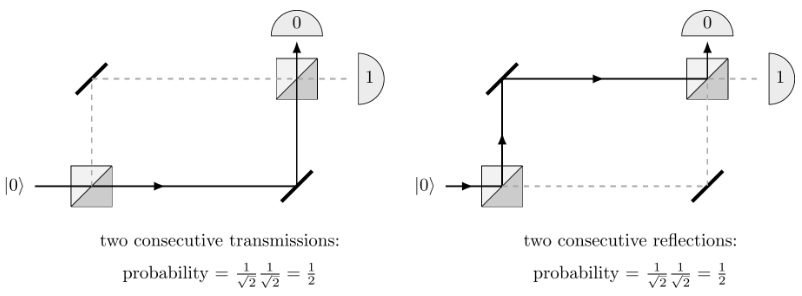
\includegraphics[width = 30em]{images/1.jpg}
\end{center}

\subsection{Classic model - which the experimental reality disagrees with!}
As illustrated, based on the classic theory, we should just add these two independent paths, each of which has a probability of $\frac{1}{2}\cdot \frac{1}{2} = \frac{1}{4}$ to happen, for a total probability of $\frac{1}{2}$ to reach the $0$ detector.

The problem with this is that the experimental observation disagrees with this prediction, as all lights fired from $\Ket{0}$ would strike the $1$ detector (and that from $\Ket{0}$ would strike the $0$ detector)

\subsection{Use probabilistic amplitude}
In fact, the action of the beam-splitter can be described by tabulating the amplitudes of transitions between its input and output ports (just like any quantum devices). Specifically for beam-splitter, we have $$
B = \begin{bmatrix}
B_{00} & B_{01}\\
B_{10} & B_{11}
\end{bmatrix} = \begin{bmatrix}
\frac{1}{\sqrt{2}} & \frac{i}{\sqrt{2}}\\
\frac{i}{\sqrt{2}} & \frac{1}{\sqrt{2}}
\end{bmatrix}
$$ (the way to understand it is \underline{reflections} have probability amplitude of $\frac{i}{\sqrt{2}}$ and \underline{transmissions} have probability amplitude of $\frac{1}{\sqrt{2}}$). The actual paths with their corresponding probability amplitudes can be illustrated as:
\begin{center}
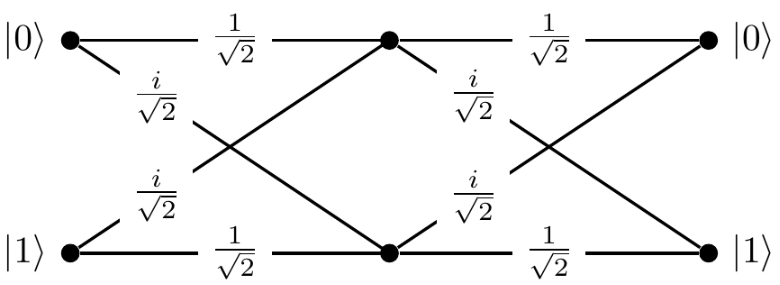
\includegraphics[width = 20em]{images/2.jpg}
\end{center}

Based on $B$, we can see that, in reality:
\begin{itemize}
    \item the \underline{probability amplitude} of a light initiated from $\Ket{0}$ to hit the $0$ detector is: $$
    \frac{1}{\sqrt{2}} \cdot \frac{1}{\sqrt{2}} + \frac{i}{\sqrt{2}} \cdot \frac{i}{\sqrt{2}} = \frac{1}{2} - \frac{1}{2} = 0
    $$, so the \underline{probability} $= |0|^2 = 0$.
    \item the \underline{probability amplitude} of a light initiated from $\Ket{0}$ to hit the $1$ detector is: $$
    \frac{1}{\sqrt{2}} \cdot \frac{i}{\sqrt{2}} + \frac{i}{\sqrt{2}} \cdot \frac{1}{\sqrt{2}} = \frac{2i}{2} = i
    $$, so the \underline{probability} $= |i|^2 = 1$.
\end{itemize}

\subsection{Finally, a simple and intuitive way}
Notice how what this beam-splitter really does is exactly a $\sqrt{\NOT}$ gate, with two such gates composed together gets us a $\NOT$ gate. The way to understand this is. But squaring (i.e. composing two gates that are the same) is also the way to get actual probabilities, so we have $$
B^2 = \begin{bmatrix}
\frac{1}{\sqrt{2}} & \frac{i}{\sqrt{2}}\\
\frac{i}{\sqrt{2}} & \frac{1}{\sqrt{2}}
\end{bmatrix}\begin{bmatrix}
\frac{1}{\sqrt{2}} & \frac{i}{\sqrt{2}}\\
\frac{i}{\sqrt{2}} & \frac{1}{\sqrt{2}}
\end{bmatrix} = \begin{bmatrix}
0 & i\\
i & 0
\end{bmatrix} = i \begin{bmatrix}
0 & 1\\
1 & 0
\end{bmatrix} = iX
$$, where $$
X = \NOT = \begin{bmatrix}
0 & 1\\
1 & 0
\end{bmatrix} \implies \sqrt{\NOT} = B = \frac{1}{\sqrt{2}} \begin{bmatrix}
1 & i\\
i & 1
\end{bmatrix}
$$

\section{Beam-splitters: quantum interference revisited}
\subsection{Mach-Zehnder Interferometer}
There are mainly two ways to alter the beam splitter model as it was shown in the first image of this talk:
\begin{itemize}
    \item Change the probability of the beam-splitter from equal probability of reflection and transmission to different (say probability amplitude of $i\sqrt{R}$ to reflect and $\sqrt{T}$ to transmit, and $R + T = 1$).
    \item Add phase shift gates on the paths like:
    \begin{center}
        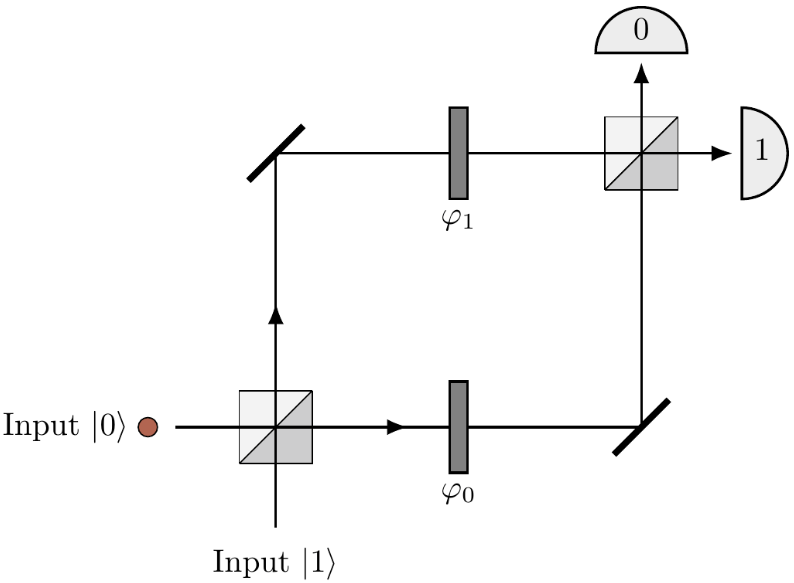
\includegraphics[width = 20em ]{images/4.jpg}
    \end{center}
\end{itemize}

Given the most general changes like listed above, we can generalize the overall $U$ vector. For example, $U_{00}$ is: $$
\begin{aligned}
    U_{00}
        &= \sqrt{T}e^{i\varphi_0}\sqrt{T} + i\sqrt{R}e^{i\varphi_1}i\sqrt{R} = Te^{i\varphi_1} - Re^{i\varphi_0}\\
\implies
    P_{00}
        &= \left|e^{i\frac{\varphi_0+\varphi_1}{2}}\prt{Te^{i\frac{\varphi_0-\varphi_1}{2}} - Re^{-i\frac{\varphi_0-\varphi_1}{2}}}\right|^2\\
        &= \left|e^{i\frac{\varphi_0+\varphi_1}{2}}\right|^2\left|Te^{i\frac{\varphi_0-\varphi_1}{2}} - Re^{-i\frac{\varphi_0-\varphi_1}{2}}\right|^2\\
        &= \prt{Te^{i\frac{\varphi_0-\varphi_1}{2}} - Re^{-i\frac{\varphi_0-\varphi_1}{2}}}\prt{Te^{-i\frac{\varphi_0-\varphi_1}{2}} - Re^{i\frac{\varphi_0-\varphi_1}{2}}}\\
        &= T^2 + R^2 - TR\prt{e^{i(\varphi_0 -\varphi_1)} + e^{-i(\varphi_0 -\varphi_1)}}\\
        &= T^2 + R^2 - 2TR\cos(\varphi_1 - \varphi_0)
\end{aligned}
$$. Similarly, we can also get $$
\begin{aligned}
    U_{10}
        &= \sqrt{T}e^{i\varphi_0}i\sqrt{R} + i\sqrt{R}e^{i\varphi_1}\sqrt{T}\\
\implies
    \sqrt{P_{10}}
        &= |i|\cdot \left|\sqrt{TR}e^{i\varphi_0} + \sqrt{TR}e^{i\varphi_1}\right| = \left|\sqrt{TR}e^{i\varphi_0} + \sqrt{TR}e^{i\varphi_1}\right|\\
    P_{10}
        &= \prt{\sqrt{TR}e^{i\varphi_0} + \sqrt{TR}e^{i\varphi_1}}\prt{\sqrt{TR}e^{-i\varphi_0} + \sqrt{TR}e^{-i\varphi_1}}\\
        &= TR\cdot 1 + TR\cdot 1 + TR\prt{e^{i(\varphi_1-\varphi_0)} + e^{-i(\varphi_1-\varphi_0)}}\\
        &= 2TR + 2TR\cos(\varphi_1-\varphi_0)
\end{aligned}
$$

\begin{proposition}[How much can, for example, $P_{00}$ vary?]
Based on $$
P_{00} = T^2 + R^2 - 2TR \cos(\varphi_1 - \varphi_0)
$$ that we have calculated above, we know that $P_{00}\in T^2 + P^2 \pm 2TR$, where $T^2 + 2TR + R^2 = (T+R)^2 = 1$ and $T^2 - 2TR + R^2 = (T-R)^2$. Furthermore, the interference term in terms of $\cos$ is clearly periodic, so, the graph may just be:
\begin{center}
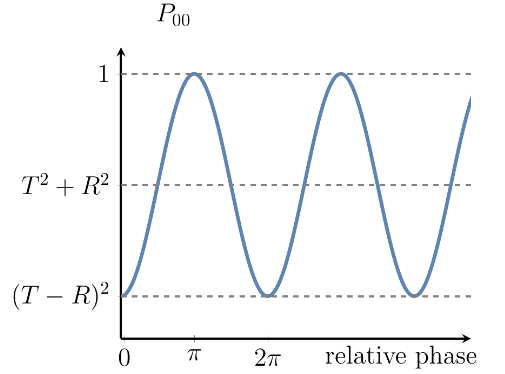
\includegraphics[width = 18em]{images/5.jpg}
\end{center}
\end{proposition}

\begin{proposition}
Light initiated by $\Ket{0}$ should reach either $1$ or $0$ detector, so the total probability should be $1$, even considering the interference.
$$
\begin{aligned}
U_{00} + U_{10}
    &= T^2 + R^2 - 2TR\cos(\varphi_1 - \varphi_0) +  2TR + 2TR\cos(\varphi_1-\varphi_0)\\
    &= T^2 + R^2 +  2TR\\
    &= (T+R)^2 = 1
\end{aligned}
$$
\end{proposition}

\begin{remark}
$U$ matrix fully describes all probability amplitude by the action of the interferometer. The most popular one is when $R = T = \frac{1}{2}$ which is fully described by $$
U = \begin{bmatrix}
-\sin \frac{\varphi_1 - \varphi_0}{2} & \cos\frac{\varphi_1 - \varphi_0}{2}\\
\cos\frac{\varphi_1 - \varphi_0}{2} & \sin \frac{\varphi_1 - \varphi_0}{2}
\end{bmatrix}
$$
\end{remark}

\section{Pauli Matrices (Revisited)}
We have defined the Pauli matrices and introduced some of their relationships and identities before. Recall that: $$
\begin{aligned}
\mathbb{1} = \begin{bmatrix}
        1 & 0\\
        0 & 1
    \end{bmatrix};
X = \begin{bmatrix}
        0 & 1\\
        1 & 0
    \end{bmatrix};
Y = \begin{bmatrix}
        0 & -i\\
        i & 0
    \end{bmatrix};
Z = \begin{bmatrix}
        1 & 0\\
        0 & -1
    \end{bmatrix}
\end{aligned}
$$

\begin{lemma}[Pauli matrices are a set of basis for $2\times 2$ matrices with $\C$ entries]\label{lemma:pauli-is-basis}
We have so far hand-waved this fact, but now we can show it more formally.
\end{lemma}
\begin{proof}
Clearly, $\left\{\begin{bmatrix}
1 & 0\\
0 & 0
\end{bmatrix}, \begin{bmatrix}
0 & 1\\
0 & 0
\end{bmatrix}, \begin{bmatrix}
0 & 0\\
1 & 0
\end{bmatrix}, \begin{bmatrix}
0 & 0\\
0 & 1
\end{bmatrix}\right\}$ is a set of basis for $2\times 2$ matrices, so it suffices for us to show that we can construct each of these by linear combinations of $\{\mathbb{1}, X, Y, Z\}$: $$
\begin{aligned}
\begin{bmatrix}
1 & 0\\
0 & 0
\end{bmatrix}
    &= \frac{1}{2}(\mathbb{1} + Z)\\
\begin{bmatrix}
0 & 1\\
0 & 0
\end{bmatrix}
    &= \frac{1}{2}(X + iY)\\
\begin{bmatrix}
0 & 0\\
1 & 0
\end{bmatrix}
    &= \frac{1}{2}(X - iY)\\
\begin{bmatrix}
0 & 0\\
0 & 1
\end{bmatrix}
    &= \frac{1}{2}(\mathbb{1} - Z)
\end{aligned}
$$
\end{proof}

\begin{theorem}
Following lemma \ref{lemma:pauli-is-basis}, we know that, given any $2\times 2$ matrix $U$, we can decompose $U$: $$
U = a_0\mathbb{1} + a_xX + a_yY + a_zZ
$$, which is just the definition of what it means to be a basis of some vector space. We have actually used this convenient identity in many places already, but now we can also discuss this further: $$
\begin{aligned}
U
    &= a_0\mathbb{1} + a_xX + a_yY + a_zZ\\
    &= \begin{bmatrix}
        a_0 + a_z & a_x - i a_y\\
        a_x + ia_y & a_0 - a_z
    \end{bmatrix}\\
    &= a_0\mathbb{1} + \vec{a}\cdot \vec{\sigma}
\end{aligned}
$$, if we denote $\vec{a} = (a_x, a_y, a_z)$, where $a_x, a_y, a_z\in \C$ and $\vec{\sigma} = (X,Y,Z) = (\sigma_x, \sigma_y, \sigma_z)$.
\end{theorem}

\begin{proposition}[$\prt{\vec{a}\cdot \vec{\sigma}}\prt{\vec{b}\cdot \vec{\sigma}} = \prt{\vec{a} \cdot \vec{b}} + i\prt{\vec{a}\times \vec{b}} \cdot \vec{\sigma}$]
\end{proposition}
\begin{proof}
$$
\begin{aligned}
\prt{\vec{a}\cdot \vec{\sigma}}\prt{\vec{b}\cdot \vec{\sigma}}
    &= \prt{(a_1 + i\alpha_1, a_2 + i\alpha_2, a_3 + i\alpha_3)(\sigma_x, \sigma_y, \sigma_z)} \prt{(b_1 + i\beta_1, b_2 + i\beta_2, b_3 + i\beta_3)(\sigma_x, \sigma_y, \sigma_z)}\\
    &= \prt{\sigma_x(a_1 + i\alpha_1) + \sigma_y(a_2 + i\alpha_2) + \sigma_z(a_3 + i\alpha_3)}\prt{\sigma_x(b_1 + i\beta_1) + \sigma_y(b_2 + i\beta_2) + \sigma_z(b_3 + i\beta_3)}\\
    &= \vec{a}\cdot \vec{b} + i\prt{\vec{a}\times \vec{b}}\cdot \vec{\sigma}
\end{aligned}
$$
\end{proof}

\begin{definition}[Inner product on this vector space of matrices as Hilbert-Schmidt product]
$$
(A\mid B) = \frac{1}{2}\Trace{A^\dag B}
$$
\end{definition}

\end{document}